\subsection{Radiation Revelations: Lengthening the Long Wire Antenna!}

\begin{tcolorbox}[colback=gray!10, colframe=black, title=E9C04] What happens to the radiation pattern of an unterminated long wire antenna as the wire length is increased? 
\begin{enumerate}[label=\Alph*.]
    \item Fewer lobes form with the major lobes increasing closer to broadside to the wire
    \item \textbf{Additional lobes form with major lobes increasingly aligned with the axis of the antenna}
    \item The elevation angle increases, and the front-to-rear ratio decreases
    \item The elevation angle increases, while the front-to-rear ratio is unaffected
\end{enumerate} \end{tcolorbox}

\subsubsection{Concepts and Explanation}

To understand the effect of increasing the length of an unterminated long wire antenna on its radiation pattern, we first need to recognize how antennas operate in general. Antennas radiate electromagnetic waves and their radiation patterns are influenced by various factors, including the antenna's length.

A long wire antenna can be described as one whose length is considerably longer than the wavelength of the signal it is transmitting or receiving. The resonances that occur in a long wire antenna lead to the formation of distinct lobes in its radiation pattern. 

As the antenna length increases:
- The number of radiation lobes in the pattern increases.
- The major lobes become more oriented along the axis of the antenna.

This helps in focusing the radiated energy in certain directions, which enhances both transmission and reception capabilities. 

To conceptualize this, let $L$ be the length of the antenna, and $\lambda$ be the wavelength:

\[
\text{Length Ratio} = \frac{L}{\lambda}
\]

If we consider the full development of the radiation pattern, with increasing $L$, we can anticipate that the number of lobes can be modeled to find out how the angle at which radiation primarily occurs changes with respect to the length ratio. As the length ratio increases, lobes appear, and the maximum radiation direction tends to align more closely with the length of the wire.

\subsubsection{Example Calculation}

Let’s assume we are working with frequencies in the HF range. If we take a frequency of 7.0 MHz, the wavelength $\lambda$ is calculated using:

\[
\lambda = \frac{c}{f}
\]

Where $c$ is the speed of light, approximately $3 \times 10^8$ m/s, and $f$ is the frequency in Hz. Thus,

\[
\lambda = \frac{3 \times 10^8}{7 \times 10^6} \approx 42.86 \text{ m}
\]

Now, if the length of our antenna is increased from, say, 10 m to 20 m, the Length Ratio changes from:

\[
\frac{10}{42.86} \approx 0.23 \quad \text{to} \quad \frac{20}{42.86} \approx 0.47
\]

With this increasing Length Ratio, we infer that the antenna will exhibit additional lobes, shifting more towards the alignment with the antenna.

\subsubsection{Diagram Representation}

A graphical representation can assist our understanding. Below is a simple graphical representation using \texttt{tikz} to illustrate typical radiation lobes for wire antennas of different lengths.

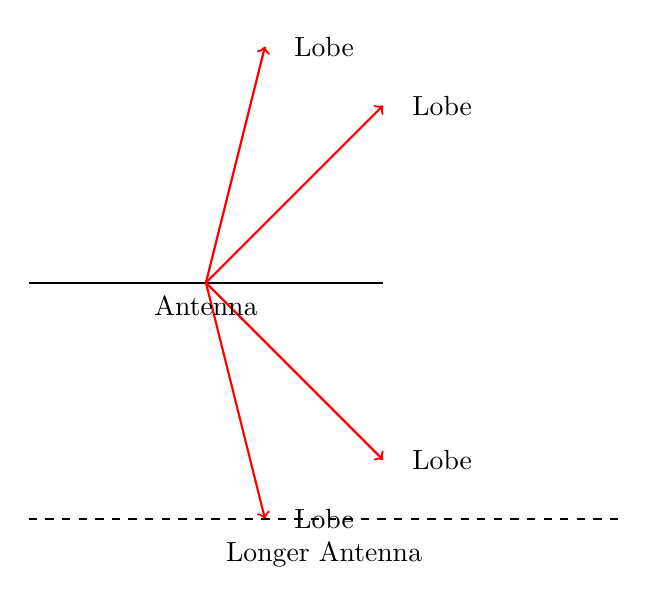
\begin{tikzpicture}[scale=1.5]
    % Draw the wire antenna
    \draw[thick] (0,0) -- (3,0);
    
    % Draw lobes for antenna at length 10m
    \draw[red, thick, ->] (1.5,0) -- (3,1.5);
    \draw[red, thick, ->] (1.5,0) -- (3,-1.5);
    \draw[red, thick, ->] (1.5,0) -- (2,2);
    \draw[red, thick, ->] (1.5,0) -- (2,-2);
    
    % Antenna label
    \node at (1.5, -0.2) {Antenna};

    % Major lobes
    \node at (3.5, 1.5) {Lobe};
    \node at (3.5, -1.5) {Lobe};
    \node at (2.5, 2) {Lobe};
    \node at (2.5, -2) {Lobe};

    % Change wire length
    \draw[thick, dashed] (0,-2) -- (5,-2);
    \node at (2.5, -2.3) {Longer Antenna};
\end{tikzpicture}

This visual supports the understanding of how increasing the length of the antenna results in more defined lobes and adjustments in the radiation pattern.
